    % !TEX root = reply_letter.tex
    \section*{Response to 2nd Referee's Comments}
    We would like to thank the Referee for his/her constructive comments, which have allowed us to considerably improve our paper. The main differences of the new version of the manuscript compared to the previous one can be found in Sections~5 and 6, Web Appendix A.2, C and D. In addition, changes regarding the specific comments have been made throughout the text.

    You may find below our responses to the specific issues raised.

    \subsection*{Major Concerns Shared by the 2nd Referee}
    \begin{enumerate}
        \item [1.] \underline{Heavier tailed negative residuals in the quantile-quantile plot.}

        We would like to thank the Referee for motivating us to check the model fit. As the Referee noted, the quantile-quantile plot for the residuals from the original model (left panel of Figure ) shows heavy tailed negative residuals. Following the suggestion of the Referee we transformed the longitudinal outcome using a $\log_2 (\mbox{PSA}+0.1)$ transformation instead of the original $\log_2 (\mbox{PSA})$ transformation. In addition, we also tried $\log_2 (\mbox{PSA}+1)$ transformation \citep{lin2000latent,pearson1994mixed}. The resulting quantile-quantile plots of the residuals in shown in Figure \ref{fig : qqplot_various_log_transform_t3}. Since the residuals from the model with $\log_2(\mbox{PSA} + 1)$ transformation met the assumptions best, we use it in the revised version of the manuscript. The corresponding longitudinal sub-model of the joint model we fit is given by:
        \begin{equation}
        \label{eq : long_model_prias_ref2}
        \begin{aligned}
    \log_2 (\mbox{PSA}_i + 1)(t) &= \beta_0 + \beta_1 (\mbox{Age}_i-70) + \beta_2 (\mbox{Age}_i-70)^2 + \sum_{k=1}^4 \beta_{k+2} B_k(t,\mathcal{K})\\ 
    &+  b_{i0} + b_{i1} B_7(t, 0.1) + b_{i2} B_8(t, 0.1) +
    \varepsilon_i(t),
    \end{aligned}
    \end{equation}
        where the error $\varepsilon_i(t)$ is assumed to be t-distributed with three degrees of freedom and scale $\sigma$.

        \begin{figure}[!htb]
        \centerline{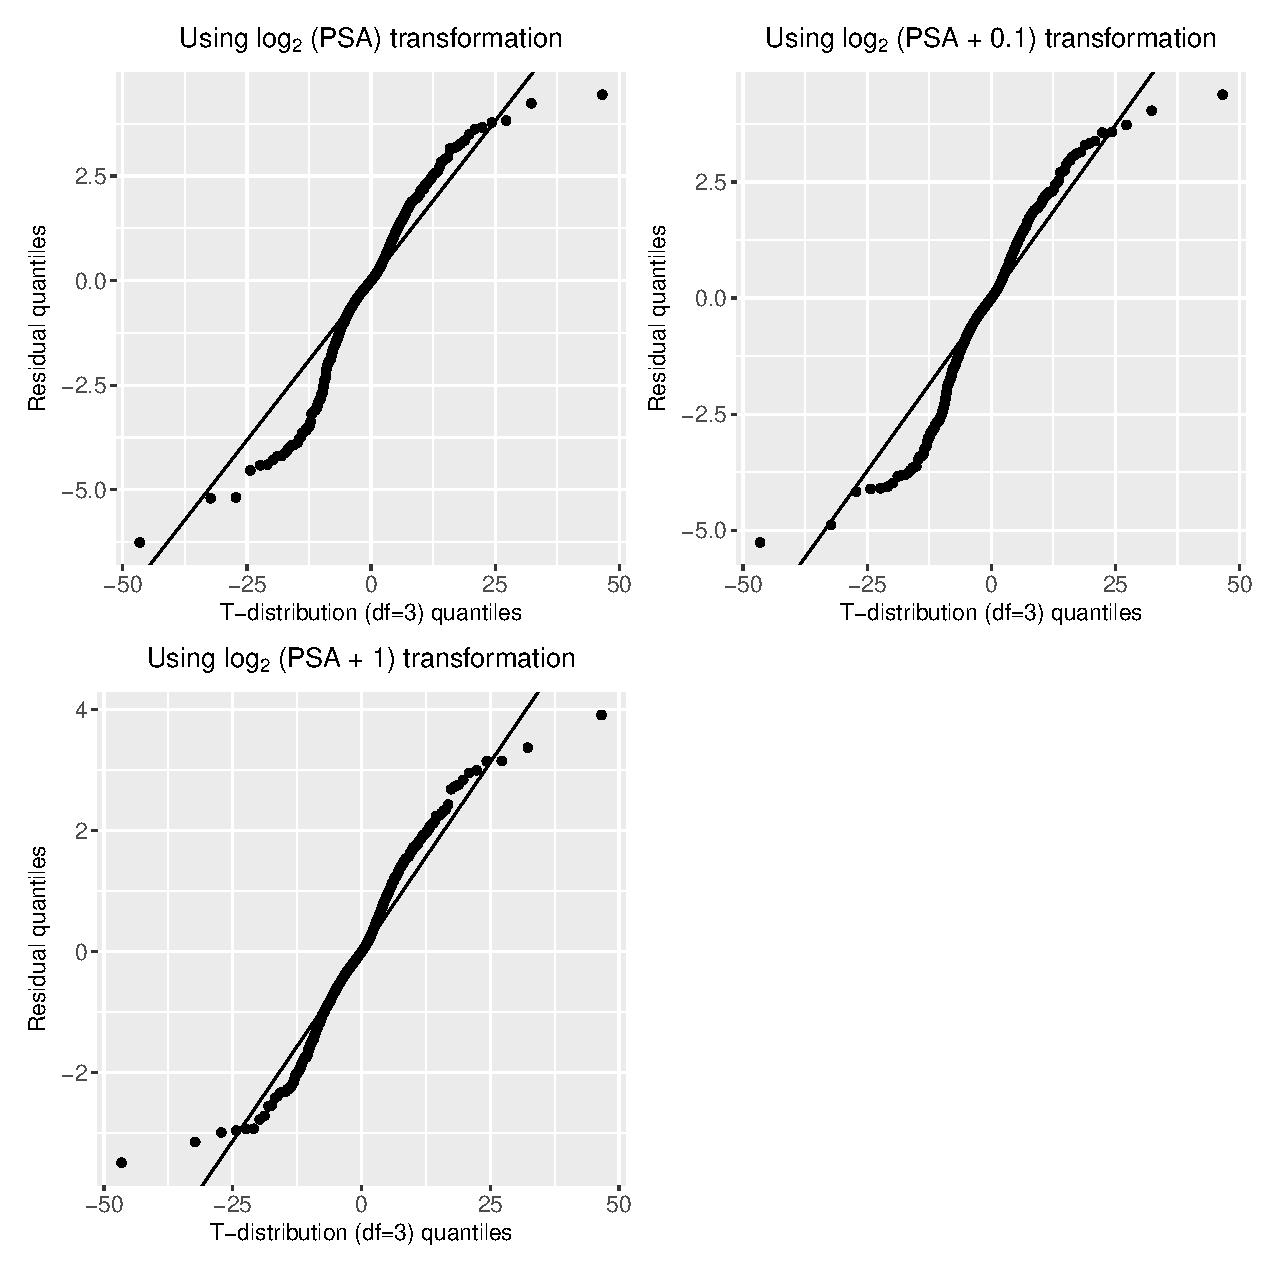
\includegraphics[width=\columnwidth]{../images/model_fit/qqplot_various_log_transform_t3.eps}}
        \caption{Quantile-quantile plots of subject specific residuals obtained from joint models with $\log_2 (\mbox{PSA})$, $\log_2(\mbox{PSA}+0.1)$, and $\log_2(\mbox{PSA}+1)$ transformed longitudinal outcome, and an assumption of t-distributed (df=3) errors, fitted to the PRIAS data set.}
        \label{fig : qqplot_various_log_transform_t3}
        \end{figure}

        
    \end{enumerate}

    \subsection*{Minor Concerns Shared by the 2nd Referee}

    \begin{enumerate}
        \item[1.] \underline{More informative captions for Table 1 and Figure 3-5.}

        We have updated the captions of Table 1 and Figure 3-5 in the revised manuscript. The revised captions along with Table/Figures are shown in Table \ref{table : sim_study_pooled_estimates} and Figure \ref{fig : meanNbVsOffset}-\ref{fig : offsetBoxPlot_all} in this reply letter.

        \item[2.] \underline{Missing subscript $i$ in Equation 7 of the original manuscript.}

        We thank the Referee for noticing this error. Equation (\ref{eq : long_model_prias_ref2}) in this reply letter shows the new equation that we use in the revised version of the manuscript.

    \end{enumerate}


        \clearpage
    \begin{figure}
    \centerline{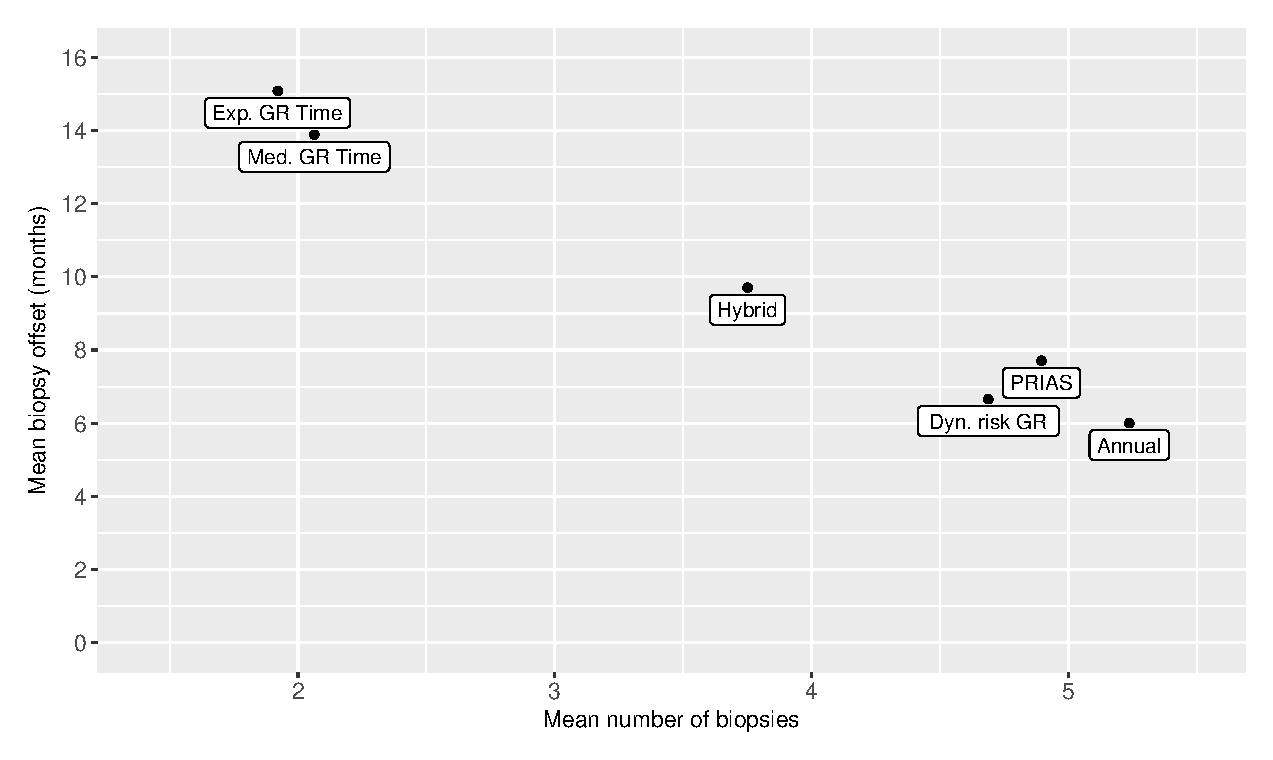
\includegraphics[width=\columnwidth]{../images/sim_study/meanNbVsOffset_all.eps}}
    \caption{Estimated mean number of biopsies conducted until PCa is detected, and mean offset (difference in time at which PCa progression is detected and the true time of PCa progression, in months) for various biopsy schedules, obtained from the simulation study with 500 simulated datasets. Types of personalized schedules: expected time of GR (Exp. GR time), median time of GR (Med. GR time), schedules based on dynamic risk of GR (Dyn. risk GR), a hybrid approach between median time of GR and dynamic risk of GR (Hybrid). Annual corresponds to a schedule of yearly biopsies and PRIAS corresponds to biopsies as per PRIAS protocol.}
    \label{fig : meanNbVsOffset}
    \end{figure}

\clearpage
    %124781 = 41484 + 41423 + 41874
    \begin{table}
    \centering
    \captionsetup{font=scriptsize}
    \caption{Estimated mean and standard deviation of the number of biopsies $N^S_j$ conducted until PCa is detected, and offset $O^S_j$ (difference in time at which PCa progression is detected and the true time of PCa progression, in months) for various biopsy schedules, obtained from the simulation study with 500 simulated datasets. Types of personalized schedules: expected time of GR (Exp. GR time), median time of GR (Med. GR time), schedules based on dynamic risk of GR (Dyn. risk GR), a hybrid approach between median time of GR and dynamic risk of GR (Hybrid). Annual corresponds to a schedule of yearly biopsies and PRIAS corresponds to biopsies as per PRIAS protocol. Patients in subgroup $G_1$ have the fastest PCa progression rate, whereas patients in subgroup $G_3$ have the slowest PCa progression rate.}
    \label{table : sim_study_pooled_estimates}
    \begin{tabular}{lrrrr}
    \Hline
    \multicolumn{5}{c}{a) All hypothetical subgroups}\\
    \hline
    Schedule          & $E(N^S_j)$ & $E(O^S_j)$ & ${\mbox{SD}(N^S_j)}$ & ${\mbox{SD}(O^S_j)}$ \\
    \hline
    Annual         & 5.24            & 6.01                & 2.53          & 3.46              \\
    PRIAS          & 4.90            & 7.71                & 2.36          & 6.31\\
    Dyn. risk GR       & 4.69            & 6.66                & 2.19           & 4.38              \\
    Hybrid       & 3.75            & 9.70                & 1.71          & 7.25              \\
    Med. GR time & 2.06            & 13.88               & 1.41          & 11.80              \\
    Exp. GR time & 1.92            & 15.08               & 1.19          & 12.11             \\
    \hline
    \multicolumn{5}{c}{b) Hypothetical subgroup $G_1$}\\
    \hline
    Schedule        & $E(N^S_j)$ & $E(O^S_j)$ & ${\mbox{SD}(N^S_j)}$ & ${\mbox{SD}(O^S_j)}$ \\
    \hline
    Annual         & 4.32            & 6.02                & 3.13          & 3.44              \\
    PRIAS          & 4.07            & 7.44                & 2.88          & 6.11    \\
    Dyn. risk GR       & 3.85            & 6.75                & 2.69          & 4.44              \\
    Hybrid       & 3.25            & 10.25               & 2.16          & 8.07              \\
    Med. GR time & 1.84            & 20.66               & 1.76          & 14.62             \\
    Exp. GR time & 1.72            & 21.65               & 1.47          & 14.75             \\
    \hline      
    \multicolumn{5}{c}{c) Hypothetical subgroup $G_2$}\\
    \hline
    Schedule        & $E(N^S_j)$ & $E(O^S_j)$ & ${\mbox{SD}(N^S_j)}$ & ${\mbox{SD}(O^S_j)}$ \\
    \hline
    Annual         & 5.18            & 5.98                & 2.13          & 3.47              \\
    PRIAS          & 4.85            & 7.70                & 2.00          & 6.29        \\
    Dyn. risk GR       & 4.63            & 6.66                & 1.82          & 4.37              \\
    Hybrid       & 3.68            & 10.32                & 1.37          & 7.45              \\
    Med. GR time & 1.89             & 12.33               & 1.16          & 9.44              \\
    Exp. GR time & 1.77            & 13.54               & 0.98          & 9.83              \\
    \hline      
    \multicolumn{5}{c}{d) Hypothetical subgroup $G_3$}\\
    \hline
    Schedule        & $E(N^S_j)$ & $E(O^S_j)$ & ${\mbox{SD}(N^S_j)}$ & ${\mbox{SD}(O^S_j)}$ \\
    \hline
    Annual         & 6.20             & 6.02                & 1.76          & 3.46              \\
    PRIAS          & 5.76             & 7.98                & 1.71         & 6.51        \\
    Dyn. risk GR       & 5.58            & 6.58                & 1.56          & 4.33              \\
    Hybrid       & 4.32            & 8.55                & 1.26          & 5.91              \\
    Med. GR time & 2.45            & 8.70                & 1.15          & 6.32              \\
    Exp. GR time & 2.27            & 10.09               & 0.99          & 7.47              \\
    \hline     
    \end{tabular}
    \end{table}

\clearpage
    \begin{figure}[!htb]
    \centerline{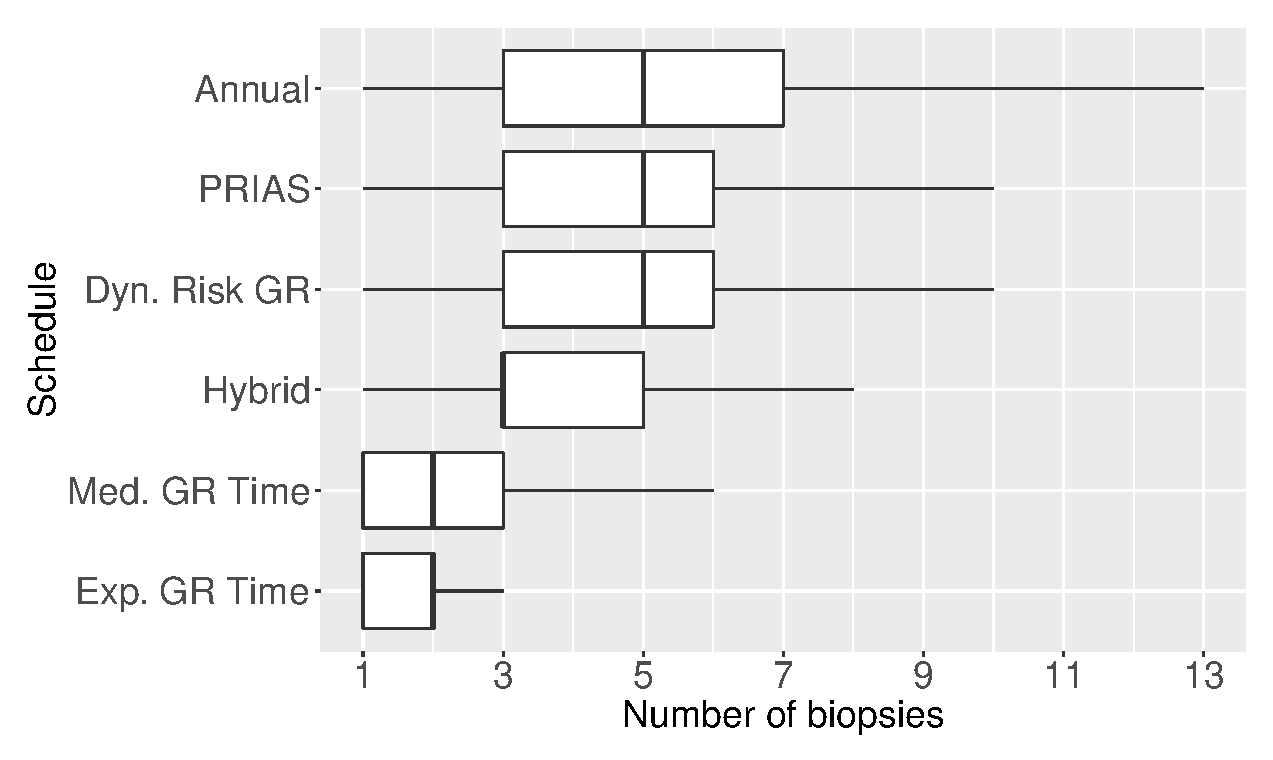
\includegraphics[width=\columnwidth]{../images/sim_study/nbBoxPlot_all.eps}}
    \caption{Boxplot showing variation in number of biopsies conducted by various biopsy schedules until PCa progression is detected, obtained from the simulation study with 500 simulated datasets. Types of personalized schedules: expected time of GR (Exp. GR time), median time of GR (Med. GR time), schedules based on dynamic risk of GR (Dyn. risk GR), a hybrid approach between median time of GR and dynamic risk of GR (Hybrid). Annual corresponds to a schedule of yearly biopsies and PRIAS corresponds to biopsies as per PRIAS protocol.}
    \label{fig : nbBoxPlot_all}
    \end{figure}

\clearpage
    \begin{figure}[!htb]
    \centerline{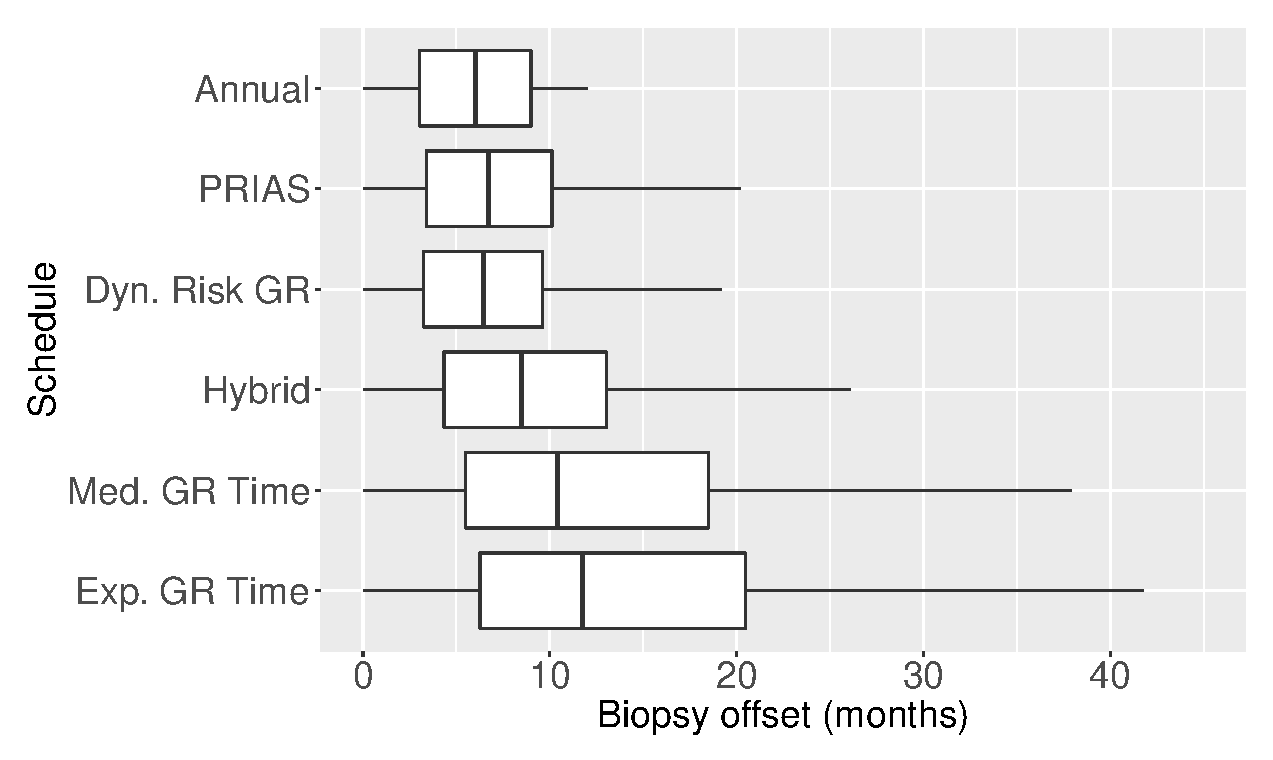
\includegraphics[width=\columnwidth]{../images/sim_study/offsetBoxPlot_all.eps}}
    \caption{Boxplot showing variation in biopsy offset (difference in time at which PCa progression is detected and the true time of PCa progression, in months) for various schedules, obtained from the simulation study with 500 simulated datasets. Types of personalized schedules: expected time of GR (Exp. GR time), median time of GR (Med. GR time), schedules based on dynamic risk of GR (Dyn. risk GR), a hybrid approach between median time of GR and dynamic risk of GR (Hybrid). Annual corresponds to a schedule of yearly biopsies and PRIAS corresponds to biopsies as per PRIAS protocol.}
    \label{fig : offsetBoxPlot_all}
    \end{figure}
        
        
